\documentclass[a4paper, 12pt]{article}
% Font and language settings
\usepackage[slovene]{babel}
\usepackage[utf8]{inputenc}
\usepackage[T1]{fontenc}
\usepackage{lmodern}
% Links
\usepackage{hyperref}
\usepackage{url}
% Images
\usepackage{graphicx}
% Better controls over figure envirnoments
\usepackage{float}
% Various math symobs
\usepackage{amssymb}
\usepackage{amsmath}
\usepackage{amsthm}
\usepackage{mathtools}
% Help with alignment
\usepackage{array}
% Multiple text columns
\usepackage{multicol}
% Miscellaneous symobls
\usepackage{wasysym}
% Custom enumeration symols
\usepackage{enumerate}
% Able to indent text with adjustwidth environment
\usepackage{changepage}
% More dashing option. Most important is \dashuline{} used for short proofs
\usepackage[normalem]{ulem}
% Better rulers for tables
\usepackage{booktabs}
% Units and unit setup
\usepackage{siunitx}
\sisetup{output-decimal-marker={,}, group-digits=false}
\usepackage{tikz}

% Comment this out if you want normal paragraph indents without empty lines between them.
% This options are set primarly for texts with a lot of shorter paragraphs, like various notes.
\setlength{\parindent}{0px}
\setlength{\parskip}{10px}

\usepackage{titlesec}
\titleformat{\section}{\bfseries\large}{}{0pt}{}

% Set title, author and date
\title{Kombinatorika}
\author{Vid Drobnič}
\date{}

\begin{document}
\maketitle
	
\section*{6b) Katera po vrsti je beseda DARILO, "ce vse permutacije zapi"semo po leksikografskem vrstenm redu.}
Spomnimo se: Leksikografski vrstni red pomeni, da so besede zapisane po abecednem vrstnem redu (tako kot v slovarju). Mi "zelimo izra"cunati koliko besed sestavljenih samo iz "crk D, A, R, I, L in O se pojavi pred besedo DARILO. Najprej si poglejmo abecedni red "crk v besedi DARILO:
\begin{center}
A, D, I, L, O, R
\end{center}
Ker so besede razvrstene po abecednem vrstem redu, bodo najprej vse besede, ki se za"cnejo s "crko A. Torej bodo pred besedo DARILO vse besede oblike A~\_~\_~\_~\_~\_. Fiksirali smo "crko A, iz ostalih 5-ih "crk pa lahko naredimo $5!$ razli"cnih besed. Torej imamo $5!$ besed, ki se za"cnejo s "crko A.

Za vsemi besedami, ki se za"cnejo s "crko A, bodo razvr"s"cene besede, ki se za"cnejo s "crko D (ker je D naslednja po abecedi). Torej bomo imeli opravkami z besedami oblike D~\_~\_~\_~\_~\_. Torej smo na prvo mesto dobili "crko, ki jo "zelimo za besedo DARILO. Poglejmo si drugo mesto.

Na drugo mesto "zelimo dati "crko A. Imamo sre"co in je ta prva po abecedi. Kar pomeni, da se ukvarjamo z besedami oblike DA~\_~\_~\_~\_. Poglejmo si tretjo "crko v besedi.

Na tretjem mestu bi si "zeleli "crko R. Ker pa so permuaticje urejene po abecedi, bodo pred njo vse besede oblike DAI~\_~\_~\_, DAL~\_~\_~\_ ter DAO~\_~\_~\_. Besed oblike DAI~\_~\_~\_ je $3!$, besed oblike DAL~\_~\_~\_ je prav tako $3!$, besed oblike DAO~\_~\_~\_ pa je spet $3!$. Sedaj smo pre"steli vse besede pred besedami oblike DAR~\_~\_~\_. Spet imamo sre"co in naslednja beseda bo DARILO, ker so I, L, O "ze po vrstenm redu.

\textbf{Povzetek:} Pred besedo DARILO so vse besede oblike A~\_~\_~\_~\_~\_, DAI~\_~\_~\_, DAL~\_~\_~\ in DAO~\_~\_~\_. Besed oblike A~\_~\_~\_~\_~\_ je $5!$, besed oblike DAI~\_~\_~\_ je $3!$, besed oblike DAL~\_~\_~\ je $3!$ in besed oblike DAO~\_~\_~\_ je $3!$. Torej je pred besedo DARILO $5! + 3! + 3! + 3! = 138$ besed. Kar pomeni, da je DARILO $139.$ beseda.

\section*{10) V zbirki imamo 5 vra"sanj iz geometrije in 7 vpra"sanj iz aritmetike. Na koliko na"cinov lahko izmed njih izberemo "stiri izpitna vpra"sanja, ki pa ne smejo biti vsa iz istega poglavja.}
Izbrati "zelimo 4 izpitna vpra"sanja iz neke zbirke. Torej se bomo ukvarjali s kombinacijami. Spomnimo se ena"cbe za izra"cun "stevila kombinacij:
\begin{equation*}
C_n^r = \dfrac{n!}{(n-r)!r!}
\end{equation*}
"Ce bi izbirali med vsemi vpra"sanji v zbirki, bi imeli na voljo 5 vpra"sanj iz geometrije in 7 iz aritmetike, kar je skupno 12 vpra"sanj. Torej bi imeli na voljo
\begin{equation*}
C_{12}^7 = 495
\end{equation*}
vpra"sanj. V te kombinacije so vklju"cene tudi kombinacije vpra"sanj samo iz poglavja aritmetike in kombinacije vpra"sanj samo iz poglavja geometrije.

V poglavju geometrije je 5 vpra"sanj. "Ce bi izbirali samo iz tega poglavja, bi imeli na voljo $C_5^4 = 5$ vpra"sanj. V poglavju aritmetike je 7 vpra"sanj. "Ce bi izbirali samo iz tega poglavja, bi imeli na voljo $C_7^4 = 35$ vpra"sanj.

Iz vseh kombinacij, ki jih lahko naredimo iz vpra"sanj iz celotne zbirke, moramo torej od"steti vse kombinacije, ki so sestavljene samo iz vpra"sanj iz poglavja geometrije in vse kombinacije, ki so sestavljene samo iz vpra"sanj iz poglavja aritmetike. Torej imamo na voljo
\begin{equation*}
C_{12}^7 - (C_5^4 + C_7^4) = 495 - (5 + 35) = 455
\end{equation*}
kombinacij vpra"sanj.

\section{12) V uradu dela 7 tehnikov, 5 laborantov in 8 in"zenirjev. Izra"cunaj, na koliko na"cinov lahko izmed sebe izberejo pet"clansko komisijo, v kateri bodo zastopane vse tri stroke.}
V komisiji nas vrstni red ne zanima, torej se bomo ponovno ukvarjali s kombinacijami. Izbiramo med $7 + 5 + 8 = 20$ ljudi. "Ce bi izra"cunali samo vse mo"zne kombinacije 5-ih ljudi iz skupine 20-tih, bi dobili $C_{20}^5 = 15504$ kombinacij. "Zal pa je pogoj, da so zastopane vse tri stroke, kar nalogo nekoliko ote"zi.

Torej moramo od na"se zgornje "stevilke nekaj od"steti. Takoj nam pride na pamet samo od"steti vse kombinacije, kjer niso zastopani tehniki, laboranti ali in"zenirji.

"Stevilo komisij, ki jih lahko naredimo, "ce niso zastopani tehniki zra"cunamo na naslednjem na"cin. Opazimo, da izbiramo samo med laboranti in in"zenirji. Torej bomo imeli na voljo 13 ljudi iz katerih bomo sestavljaji komisi 5-ih "clanov. To je $C_{13}^5 = 1287$ mo"znih kombinacij. V te kombinacije so vklju"cene tudi vse kombinacije kjer so zastopani samo laboranti ali pa samo in"zenirji.

"Stevilo komisij, ki jih lahko naredimo, "ce niso zastopani laboranti izra"cunamo podobno kot prej. To je $C_{15}^5 = 3003$ mo"znih kombinacij.

"Stevilo komisij, ki jih lahko naredimo, "ce niso zastopani in"zenirji spet izra"cunamo na podoben na"cin. To je $C_{12}^5 = 792$ mo"znih kombinacij.

Torej od vseh kombinacij od"stejemo "stevilo kombinacij kjer niso zastopane vse stroke in dobimo:
\begin{equation*}
C_{20}^5 - (C_{13}^5 + C_{15}^5 + C_{12}^5) = 15504 - (1287 + 3003 + 792) = 10 422
\end{equation*}
"Zal pa "se nismo kon"cali, saj smo od"steli nekoliko preve"c. Poglejmo, kaj moramo pri"steti nazaj.

Ko smo izra"cunali "stevilo mo"znih komisij samo s tehniki in laboranti, s bile v teh kombinacijah tudi komisije, kjer so bili samo tehniki, ali pa samo laboranti. Ko smo potem izra"cunali "se "stevilo komisij samo s tehniki in in"zenirji, so bile v teh kombinacijah tudi kombinacije, kjer so bili v komisiji samo tehniki ali pa samo in"zenirji. Z metodo ostrega pogleda opazimo, da sem v zgornjih dveh povedih dvakrat omenil komisije v katerih nastopajo samo tehniki. To pomeni, da smo dvakrat od"steli kombinacije, kjer so v komisiji samo tehniki, od"steti pa bi jih bilo potrebno samo enkrat. Podobno velja za komisije iz samih laborantov in za komisije iz samih in"zenirjev. Pri"steti je torej treba kombinacije kjer je komisija sestavljena iz samih laborantov, tehnikov ali in"zenirjov. "Stevilo kombinacij pet"clanske komisij iz sedmih tehnikov je $C_7^5 = 21$ Podobno naredimo z laboranti in in"zenirji in dobimo:
\begin{equation*}
10 422 + C_7^5 + C_5^5 + C_8^5 = 10422 + 21 + 1 + 56 = 10500
\end{equation*}
Odgovor je torej, da lahko komisijo sestavimo na 10500 mo"znih na"cinov.

\section{18) Na kro"znici le"zi 12 to"ck. Pove"zemo jih z dalicami, ki se za"cnejo v eni in kon"cajo v drugi od teh 12 to"ck.}
\subsection*{a) Koliko daljic dolo"cajo te to"cke}
"Ce si nari"semo skico opazimo, da lahko iz vsake to"cke vle"cemo 11 daljic. Ker imamo 11 to"ck je to torej $12 \cdot 11$ daljic. "Zal pa se nekatere daljice na tak na"cin podvojijo. "Ce smo iz to"cke $A$ vlekli daljico v to"cko $B$ smo nato "steli se primer kjer smo vlekli daljico iz to"cke $B$ v $A$. Vsako daljico smo "steli dvakrat. Rezultat bo torej:
\begin{equation*}
\dfrac{12 \cdot 11}{2} = 66
\end{equation*}

\subsection*{b) Koliko trikotnikov dolo"cajo te to"cke}
Za  trikotnik potrebujemo 3 to"cke. Torej si lahko iz 12 to"ck izberemo 3 in nari"semo trikotnik, ki je dolo"cen z izbranimi to"ckami. Ker izbiramo 3 to"cke iz 12-ih in nas ne zanima vrstni red, nas to spomnija na kombinacije. Odgovor je torej $C_{12}^3 = 220$ trikotnikov.

\section*{19) V ravnini le"zi snop 10 vzporednih premic. Te vzporednice seka drug snop, ki ga sestavlja 8 vzporednic (tudi te le"zijo v isti ravnini). Izra"cunaj, koliko paralelogramov dolo"cajo te premice.}
Za paralelogram potrebujemo 4 daljice, ki pa so paroma vzporedne. Prvi snop ima 10 vzporednih premic. "Ce izberemo 2 premici iz tega snopa imamo "ze 2 nosilki stranic nekega paralelograma. Potrebujemo "se drugi dve nosilki daljic. Te bomo izbirali v drugem snopu, ki ima 8 vzporednih premic. Ker nas vrstni red ne zanima, se bomo ukvarjali s kombinacijami. "Ce izberemo 2 premici iz prvega snopa, bomo dobili $C_{10}^2 = 45$ mo"znih kombinacij. Iz drugega snopa bomo prav tako izbrali 2 premici. To pomeni, da lahko iz drugega snopa dobimo $C_8^2 = 28$ mo"znih kombinacij.

Ker lahko za vsaki dve izbrani premici iz prvega snopa izberemo katerikoli dve premici iz drugega snopa, bomo "stevilo mo"znih kombinacij zmno"zili med sabo. Torej je "stevilo vseh mo"znih paralelogramov:
\begin{equation*}
C_{10}^2 \cdot C_8^2 = 45 \cdot 28 = 1260
\end{equation*}
Odgovor je, da te premice dolo"cajo 1260 paralelogramov.

\section{20) Koliko razli"cnih zneskov lahko pla"ca"s, "ce ima"s pri sebi en kovanec za 10 centov, en kovanec za 20 centov, enkovanec za 50 centov, en kovanec  za 1 evro in en kovanec za 2 evra?}
Pri sebi imamo pet razli"cnih kovancev. Pla"camo lahko z enim, dvema, tremi, "stirimi ali petimi kovanci. Ker so vsi kovanci razli"cni, bo vsaka kombinacija kovancov pridelala drug znesek. Z metodo ostrega pogleda opazimo, da je opomba v resnici namig in da se bomo ukvarjali s kombinacijami.

"Ce pla"camo z enim kovancem, imamo na voljo $C_5^1$ razli"cnih kombinacij kovancev, kar pomeni da imamo $C_5^2$ razli"cnih vrednosti. "Ce pla"camo z dvema kovancema, imamo na voljo $C_5^2$ razli"cnih kombinacij kovancev, kar pomeni da imamo $C_5^2$ razli"cnih vrednosti. Podobno naredimo za tri, "stiri in pet kovancev. Torej je skupno "stevilo razli"cnih zneskov, ki jih lahko pla"camo:
\begin{equation*}
C_5^1 + C_5^2 + C_5^3 + C_5^4 + C_5^5 = 5 + 10 + 10 + 5 + 1 = 31
\end{equation*}
\textbf{Opomba:} matematik v meni si ne more pomagati, da ne bi zgornje vsote zapisal na kraj"se, zato zgolj samo kot zanimivost povem, da lahko zgornjo ena"cbo zapi"semo kot:
\begin{equation*}
\sum_{n=1}^{5} C_5^n = 31
\end{equation*}

\section{22) V bobnu za "zrebanje so "zogice ozna"cene s celimi "stevili od 1 do 20 (vklju"cno). Iz bobna iz"zrebamo dve "stevili hkrati. Izra"cunaj verjetnost, da je vsota obeh "stevil enaka 16.}
Iz navodil lahko razberemo, da imamo na voljo 20 "zogic. Torej je "stevilo vseh mo"znosti enako:
\begin{equation*}
n = C_{20}^2 = 190
\end{equation*}
\textbf{Opomba:} ne spomnim se, kako v srednji "soli u"cijo te oznake, zato so moje oznake verjetno druga"cne od tistih v zvezku in u"cbeniku.

Da je vsota obeh "zogic enaka 16, moramo potegniti eno izmed naslednjih mo"znosti:
\begin{table}[!htbp]
	\centering
	\begin{tabular}{c|c}
		1 & 15 \\
		2 & 14 \\
		3 & 13 \\
		4 & 12 \\
		5 & 11 \\
		6 & 10 \\
		7 & 9
	\end{tabular}
\end{table}

Opazimo, da je teh mo"znosti 7, torej sledi $k=7$. Verjetnost torej izra"cunamo:
\begin{equation*}
P(A) = \dfrac{k}{n} = \dfrac{7}{190} \approx 3,68\%
\end{equation*}

\section{23) Kolo sre"ce ima na obodu cela "stevila od 1 do 20 (vklju"cno). Kolo sre"ce zavrtimo dvakrat in tako dobimo dve "stevili. Izra"cunaj verjetnost, da je vsota obeh "stevil enaka 16.}
Naloga je zelo podobna prej"snji, vendar ima nekaj sprememb. Ko kolo zavrtimo prvi"c, imamo mo"znih 20 razli"cnih izidov. Ko kolo zavrtimo drugi"c, imamo mo"znih prav tako 20 izidov. "Stevilo mo"znosti je torej enako:
\begin{equation*}
n = 20 \cdot 20 = 400
\end{equation*}

"Zelimo, da je vsota obeh "stevil enaka 16. Za to se mora zgoditi eden od naslednjih izidov:
\begin{table}[!htbp]
	\centering
	\begin{tabular}{c|c}
		\textbf{Prvo "stevilo} & \textbf{Drugo "stevilo} \\ \hline
		1 & 15 \\
		2 & 14 \\
		3 & 13 \\
		4 & 12 \\
		5 & 11 \\
		6 & 10 \\
		7 & 9 \\ 
		8 & 8 \\
		9 & 7 \\
		10 & 6 \\
		11 & 5 \\
		12 & 4 \\
		13 & 3 \\
		14 & 2 \\
		15 & 1
	\end{tabular}
\end{table}

Teh mo"znosti je 15. Iz tega sledi $k = 15$. Verjetno je torej:
\begin{equation*}
P(A) = \dfrac{k}{n} = \dfrac{15}{400} \approx 3,75\%
\end{equation*}

\section*{24) V posodi je pet belih "zogic, tri "crne in dve zeleni. Iz posode na slepo vzamemo tri "zogice hkrati. Izra"cunaj verjetno naslednjih dogodkov in jih zaokro"zi na stotinko procenta}
V obeh dogodkih bo na"s $n$ enak. Ker izvle"cemo tri "zogice iz skupine 5 belih, 3 "crnih in 2 zeleni, bo "stevilo vseh "zogic 10, in $n = C_{10}^3 = 120$.
\subsection*{$A$: to"cno ena od izvle"cenih "zogic je bela}
"Ce more biti to"cno ena izmed izvle"cenih "zogic bela, morata biti ostali dve "crni ali pa zeleni. To pomeni, da moramo izbrati eno izmed petih belih "zogic. Za vsako belo "zogico, ki jo izvle"cemo imamo na voljo "se vse kombinacije zelenih in "crnih "zogic. Teh kombinacij je $C_5^5 = 10$. "Stevilo ugodnih dokodkov $k$ je torej:
\begin{equation*}
k = 5 \cdot C_5^2 = 50
\end{equation*}
Verjetnost dogodka $A$ izra"cunamo slede"ce:
\begin{equation*}
P(A) = \dfrac{k}{n} = \dfrac{50}{120} \approx 41,67\%
\end{equation*}

\subsection*{$B$: vsaj dve od izvle"cenih "zogic sta "crni}
To pomeni, da mora biti "stevilo "crnih izvle"cenih "zogic enako 2 ali 3. Ugodni so torej dogodki, kjer izvle"cemo 2 "crni "zogici, in eno "zogico, ki je bela ali zelena in dogodki kjer izvle"cemo 3 "crne "zogice. 

Za vsaki 2 "crni "zogici, lahko izvle"cemo katerokoli kombinacijo belih in zelenih "zogic. "Stevilo dogodkov, kjer izvle"cemo 2 "crni "zogici je torej $C_3^2 \cdot C_7^1$.

"Stevilo dogodkov kjer izvle"cemo 3 "crne "zogice je $C_3^3$.

"Stevilo vseh ugodnih dogodkov $k$ je torej:
\begin{equation*}
k = C_3^2 \cdot C_7^1 + C_3^3 = 22
\end{equation*}
Verjetnost dogodka $B$ potemtakem izra"cunamo:
\begin{equation*}
P(B) = \dfrac{k}{n} = \dfrac{22}{120} \approx 18,33\%
\end{equation*}

\subsection*{$C$: Vse tri izvle"cene "zogice so enake barve}
To pomeni, da moramo izvle"ci 3 bele "zogice, ali 3 "crne "zogice ali 3 zelene "zogice. Zelenih "zogici sta samo dve, torej ni mo"zno izvle"ci treh zelenih "zogic. "Stevilo dogodkov kjer izvle"cemo 3 zelene "zogice je torej 0, "Stevilo dogodkov, kjer izvle"cemo 3 bele "zogice je $C_5^3$, "stevilo dogodkov kjer izvle"cemo 3 "crne "zogice je $C_3^3$. "Stevilo vseh ugodnih dogodkov $k$ je torej:
\begin{equation*}
k = C_3^3 + C_5^3 + 0 = 1 + 10 + 0 = 11
\end{equation*}
Verjetnost dogodka $C$ je torej:
\begin{equation*}
P(C) = \dfrac{k}{n} = \dfrac{11}{120} \approx 9,17\%
\end{equation*}

\section*{25) V razredu je 11 fantov (eden od njih je Ro"zle) in 16 deklet (ena od njih je "Spela) Izmed njih iz"zrebamo "stiri"clansko delagacijo. Izra"cunaj verjetnosti naslednjih dogodkov.}
Tako kot pri prej"snji nalogi, bo tudi tukaj $n$ enak za vse dogodke. V razredu je 27 u"cencev, izmed katerih izbiramo "stiri. $n$ je torej $n = C_{27}^4 = 17550$.

\subsection*{$A$: v delagaciji sta tudi Ro"zle in "Spela}
V delagaciji morata biti ro"zle in "spela. Torej imamo na voljo "se 10 fantov in 15 deklet, kar je 25 u"cencev. Dva smo "ze izbrali (Ro"zleta in "Spelo). Izbrati moramo torej "se dva. "Stevilo ugodnih dogodkov $k$ je torej $k = C_{25}^2 = 300.$. Verjetnost dogodka $A$ izra"cunamo:
\begin{equation*}
P(A) = \dfrac{k}{n} = \dfrac{300}{17550} \approx 1,71\%
\end{equation*}

\subsection*{$B$: v delagaciji je to"cno eden od njiju}
V delagaciji je torej Ro"zle ali "Spela, ne pa oba skupaj.

"Ce je v delagaciji Ro"zle, imamo na voljo "se 10 fantov med katerimi izbiramo. Prav tako imamo na voljo samo 15 deklet, saj "Spele ne smemo izbrati. Izbirali bomo torej tri u"cence izmed 25-ih. "Stevilo dogodkov, kjer je v delagaciji Ro"zle je torej $C_{25}^3$.

"Ce je v delagaciji "Spela, imamo na voljo "se 15 deklet in 10 fantov, saj Ro"zleta ne smemo izbrati. Izbirali bomo ponovno kot prej, trei u"cence med 25-imi. "Stevilo dogodkov, kjer je v delagaciji Ro"zle je torej $C_{25}^3$.

Skupno "stevilo ugodnih dogodkov je "stevilo dogodkov kjer je v delagaciji to"cno Ro"zle, ali pa to"cno "Spela. $k$ torej izra"cunamo slede"ce:
\begin{equation*}
k = C_{25}^3 + C_{25}^3 = 4600
\end{equation*}
Verjetnost dogodka $B$ je torej:
\begin{equation*}
P(B) = \dfrac{k}{n} = \dfrac{4600}{17550} \approx 26,21\%
\end{equation*}

\subsection*{$C$: "Spela je edina "zenska v delegaciji}
V delagaciji bo torej "Spela in "se trije fantje. To pomeni, da bomo izbirali samo med 11-timi fanti. "Stevilo ugodnih dogodkov $k$ je torej $k = C_{11}^3 = 165$.

Verjetnost dogodka $C$ torej izra"cunamo:
\begin{equation*}
P(C) = \dfrac{k}{n} = \dfrac{165}{17550} \approx 0,94\%
\end{equation*}

\section*{26) Na "soli je 144 u"cencev. U"ceni lahko obiskujejo fizikalni, biolo"ski in kemijski kro"zek. Fizikalni kro"zek obiskuje 41 u"cencev, biolo"ski kro"zek obiskje 37 u"cencev, kemijski kro"zek pa 42 u"cencev. Fizikalni in biolo"ski kro"zek obiskuje 14 u"cencev. Biolo"ski in kemijski kro"zek obiskuje 16 u"cencev. Kemijski in fizikalni kro"zek obiskuje 18 u"cencev. Vse tri kor"zke obiskuje 10 u"cencev. Na slepo izberemo enega od u"cencev s te "sole.}
Ne glede na podnalogo bo "stevilo vseh mo"znih dogodkov $n$ enako. Enega u"cenca izberemo izmed 144-ih, torej je $n = C_{144}^1 = 144$.

Ta naloga bi bila zelo trivialna, "ce bi vedeli to"cno koliko u"cencev obiskuje samo fizikalni kro"zek, koliko samo fizikalni in biolo"ski, koliko samo fizikalni in kemisjki in koliko jih obiskuje vse tri. Podatki pa so podani tako, da se prekrivajo. Za la"zjo predstavo si lahko nari"semo Vennov diagram.
\begin{figure}[!htbp]
	\centering
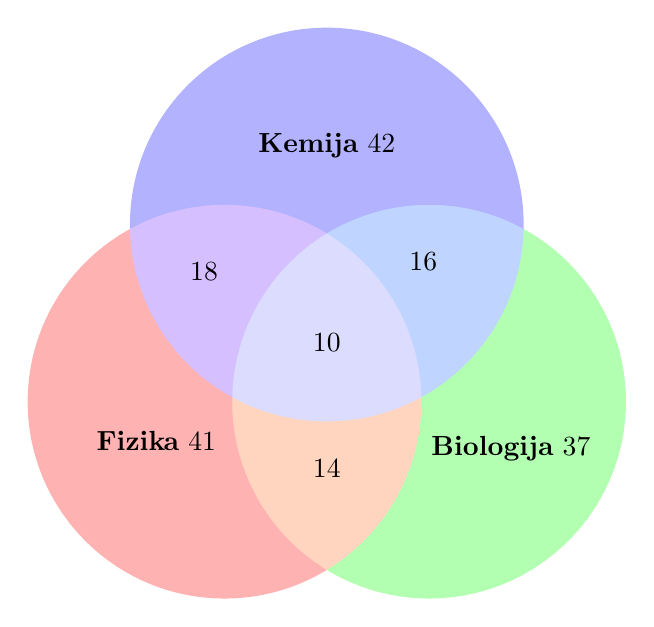
\begin{tikzpicture}
	\begin{scope}[blend group=soft light]
		\fill[blue!30] (90:1.5) circle(2.5);
		\fill[red!30] (210:1.5) circle(2.5);
		\fill[green!30] (330:1.5) circle(2.5);
	\end{scope}
	\node at (90:2.5) {\textbf{Kemija} 42};
	\node at (210:2.5) {\textbf{Fizika} 41};
	\node at (330:2.7) {\textbf{Biologija} 37};
	\node {10};
	\node at (150:1.8) {18};
	\node at (40:1.6) {16};
	\node at (270:1.6) {14};
\end{tikzpicture}
\caption{Vennov diagram u"cencev}
\end{figure}

Iz diagrama vidimo, da npr.\,fizikalni in biolo"ski kro"zek obiskuje 14 u"cencev, 10 od teh u"cencev pa obiskuje vse tri kro"zke. Torej je "stevilo u"cencev, ki obiskuje samo fizikalni in biolo"ski kro"zek enako 4. Podobno lahko naredimo za drugi dve kombinaciji kro"zkov.

Na podoben na"cin lahko izra"cunamo koliko u"cencev obiskuje npr.\,samo fizikalni kro"zek. Samo kemijski in fizikalni obiskuje 8 u"cencev, samo fizikalni in biolo"ski obiskujejo 4 u"cenci, vse tri kro"zke pa obiskuje 10 u"cencev. "Ce fizikalni kro"zek obiskuje 41 u"cencev, potemtakem samo fizikalni kro"zek obiskuje $41 - 4 - 8 - 10 = 19$ u"cencev.

Na tak na"cin lahko izra"cunamo "se koliko u"cencev obiskuje samo druga dva kro"zka. Kon"cni izra"cun nas pripelje do naslednjih "stevilk:
\begin{table}[!htbp]
	\centering
	\begin{tabular}{c|c|c|c|c|c|c}
		\textbf{K} & \textbf{F} & \textbf{B} & \textbf{K \& B} & \textbf{K \& F} & \textbf{F \& B} & \textbf{K \&F \& B} \\ \hline
		18 & 19 & 17 & 6 & 8 & 4 & 10
	\end{tabular}
\end{table}

\subsection*{$A$: izbrani u"cenec obiskuje to"cno en kro"zek}
To pomeni, da mora izbrani u"cenec obiskovati samo kemijo, samo fiziko, ali pa samo biologijo. Iz zgornje tabele preberemo, da samo kemijo obiskuje 18 ljudi, samo fiziko 19 ljudi, samo biologijo pa 17 ljudi. Torej moramo izbrati enega u"cenca izmed $18  + 19 + 17 = 54$. Ugodnih dogodkov $k$ je torej $k = C_{54}^1 = 54$.

Verjetnost dogodka $A$ se izra"cuna:
\begin{equation*}
P(A) = \dfrac{k}{n} = \dfrac{54}{144} = 37,5\%
\end{equation*}

\subsection*{$B$: izbrani u"cenec obiskuje to"cno dva kro"zka}
Izbrani u"cenec mora obiskovati samo kemijo in fiziko, samo kemijo in biologijo, ali pa samo fiziko in biologijo. Iz zgornje tabele preberemo, da je u"cencov, ki ustrezajo tem pogojem $8 + 6 + 4 = 18$. Ugodnih dogodkov $k$ je torej $k = C_{18}^1 = 18$.

Verjetnost dogodka $B$ se izra"cuna:
\begin{equation*}
P(B) = \dfrac{k}{n} = \dfrac{18}{144} = 12,5\%
\end{equation*}

\section*{27) Doma imamo tri matemati"cne, dva kemijska in tri fizikalne priro"cnike. Ne da bi pazili na vrstni red, jih zlo"zimo na polico. Izra"cunaj, kolik"sna je verjetnost, da bodo matemati"cni priro"cniki skupaj, kemijski skupaj in fizikalni skupaj. Rezultat zaokro"zi na tri mesta.}
Skupaj imamo 8 priro"cnikov. Ko jih zlo"zimo na polico, nas vrstni red zanima, torej imamo opravka s permutacijami. "Stevilo vseh dogodkov je enako "stevilo na"cinov na katere lahko zlo"zimo priro"cnike na polico. Ker je priro"cnikov 8, je potem "stevilo vseh dogodkov $m = 8!$.

\begin{figure}[!htbp]
	\centering
	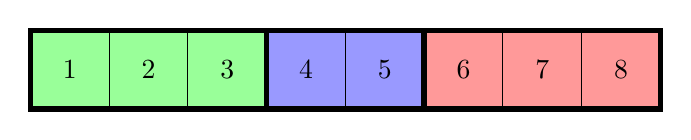
\begin{tikzpicture}
		\draw [line width=2pt, fill=green!40] (0, 0) rectangle (3, 1);
		\draw [line width=2pt, fill=blue!40] (3, 0) rectangle (5, 1);
		\draw [line width=2pt, fill=red!40] (5, 0) rectangle (8, 1);

		\draw (1, 0) -- (1, 1);
		\draw (2, 0) -- (2, 1);
		\draw (4, 0) -- (4, 1);
		\draw (6, 0) -- (6, 1);
		\draw (7, 0) -- (7, 1);

		\foreach \x in {1, ..., 8} {
			\node at (\x - 0.5, 0.5) {\x};
		}
	\end{tikzpicture}
	\caption{Polica s priro"cniki}
	\label{img:polica}
\end{figure}

Na sliki~\ref{img:polica} opazimo, da imamo tri skupine priro"cnikov. Zelena skupina nam predstavlja matemati"cne priro"cnike, modra kemijske, rde"ca pa fizikalne. Poglejmo si bolj podrobno matemati"cne priro"cnike. "Ce bi na polico zlo"zili samo matemati"cne priro"cnike, bi jih lahko zlo"zili na $3!$ na"cinov (trije so in zanima nas vrstni red, zaradi "cesar uporabimo permutacije). Podobno lahko naredimo za kemijske in fizikalne priro"cnike.

V zgornji sliki so matemati"cni priro"cniki zeleni in ozna"ceni s "stevili $1, 2$ in $3$. Ta "stevila lahko med sabo ,,me"samo'', oziroma bolj natan"cno: zelenim (matemati"cnim) priro"cnikom lahko zamenjamo vrstni red. Torej je "stevilo mo"znih vrstnih redov priro"cnikov v zeleni skupini $3!$. Podobno velja za kemijske in fizikalne priro"cnike.

"Ce bi me"sali samo vrstni red priro"cnikov, bi torej dobili "stevilo razli"cnih vrstnih redov $3! \cdot 2! \cdot 3!$. Poglejmo zakaj uporabimo mno"zenje in ne se"stevanje. Za la"zje razumevanje se osredoto"cimo samo na zelene in modre priro"cnike in dobimo naslednjo skico:
\begin{figure}[!htbp]
	\centering
	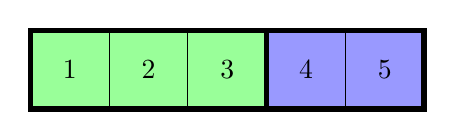
\begin{tikzpicture}
	\draw [line width=2pt, fill=green!40] (0, 0) rectangle (3, 1);
	\draw [line width=2pt, fill=blue!40] (3, 0) rectangle (5, 1);
	
	\draw (1, 0) -- (1, 1);
	\draw (2, 0) -- (2, 1);
	\draw (4, 0) -- (4, 1);
	
	\foreach \x in {1, ..., 5} {
		\node at (\x - 0.5, 0.5) {\x};
	}
	\end{tikzpicture}
\end{figure}

Za vsak poljuben vrstni red zelenih priro"cnikov, lahko modre priro"cnike razporedimo na $2!$ razli"cnih na"cinov. Torej "ce so zeleni priro"cniki v vrtnem redu $1, 2, 3$, dobimo naslenjo skico:
\begin{figure}[!htbp]
	\centering
	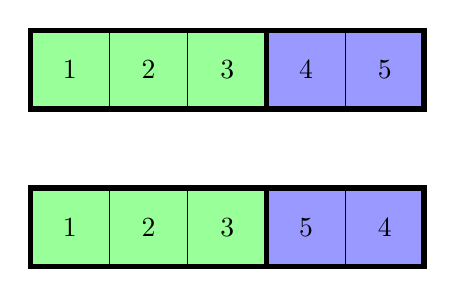
\begin{tikzpicture}
	\draw [line width=2pt, fill=green!40] (0, 0) rectangle (3, 1);
	\draw [line width=2pt, fill=blue!40] (3, 0) rectangle (5, 1);
	
	\draw (1, 0) -- (1, 1);
	\draw (2, 0) -- (2, 1);
	\draw (4, 0) -- (4, 1);
	
	\foreach \x in {1, ..., 5} {
		\node at (\x - 0.5, 0.5) {\x};
	}

	\draw [line width=2pt, fill=green!40] (0, -2) rectangle (3, -1);
	\draw [line width=2pt, fill=blue!40] (3, -2) rectangle (5, -1);

	\draw (1, -2) -- (1, -1);
	\draw (2, -2) -- (2, -1);
	\draw (4, -2) -- (4, -1);

	\foreach \x in {1, ..., 3} {
		\node at (\x - 0.5, -1.5) {\x};
	}

	\node at (4 - 0.5, -1.5) {5};
	\node at (5 - 0.5, -1.5) {4};
	\end{tikzpicture}
\end{figure}

Ker lahko to naredimo za vsak vrstni red zelenih, bi dobili $3! \cdot 2!$ mo"znih razporeditev. "Zal pa "se nismo popolnoma kon"cali. Na vsako skupino priro"cnikov lahko gledamo tudi iz vidika skupina. Torej namesto, da se ukvarjamo z vrstnim redom priro"cnikov v recimo zeleni skupini, si lahko pogledamo tudi vrstni red skupin. Poenostavljeno: zami"zimo na eno oko in se pretvarjamo, da skupina priro"cnikov ni sestavljena iz posame"cnih priro"cnikov. To vidimo na skici~\ref{fig:skupine}.

\begin{figure}[!htbp]
	\centering
	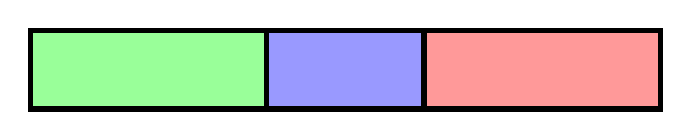
\begin{tikzpicture}
	\draw [line width=2pt, fill=green!40] (0, 0) rectangle (3, 1);
	\draw [line width=2pt, fill=blue!40] (3, 0) rectangle (5, 1);
	\draw [line width=2pt, fill=red!40] (5, 0) rectangle (8, 1);
	\end{tikzpicture}
	\caption{Skica posame"cnih skupin}
	\label{fig:skupine}
\end{figure}

Te skupine lahko med sabo preme"samo na nadaljnih $3!$ razli"cnih na"cinov (ker imamo tri elemente in se spet ukvarjamo s permutacijami). To pomeni, da lahko damo npr.\,skupino fizikalnih priro"cnikov pred matemati"cne. Poglejmo "se, kaj to pomeni v "stevilkah.

Malo prej smo nara"cunali, da "ce spreminjamo vrstni red knjig v posame"cni skupini, dobimo $3!\cdot 2!\cdot 3!$ mo"znosti. Ravnokar smo ugotovili, da je "se $3!$ mo"znosti razporeditve skupin. Te dve stvari ponovno zdru"zimo z mno"zenjem in dobimo, da je "stevilo ugodnih dogodkov $k = 3! \cdot (3! \cdot 2! \cdot 3!)$. Operacijo mno"zenja uporabimo zaradi podobnega argumenta kot prej. Za vsak izbran vrstni red posame"cnih skupin na polici, lahko spreminjamo vrstni red posame"cnih knjig v posame"cni polici. Za doma"co nalogo in bolj"se razumevanje, se lahko doma poigramo s fizi"cnimi knjigami oziroma zvezki.

Sedaj moramo izra"cunati "se verjetnost. Torej samo vstavimo nara"cunane "stevilke v formulo:
\begin{equation*}
P(A) = \dfrac{k}{n} = \dfrac{8!}{3! \cdot (3! \cdot 2! \cdot 3!)} = \dfrac{3}{280} \approx 1,07\%
\end{equation*}

\section*{28) Na svetovnem prvenstvu v balinanju sodeluje 10 dr"zav, med njimi tudi Slovenija in Mad"zarska. Organizatorji bodo razdelili sodelujo"ce dr"zave z "rebom v dve skupini po 5 dr"zav. Izra"cunaj verjetnost, da bosta Slovenija in Mad"zarska v isti skupini. Rezultat zaokro"zi na "stiri mesta.}
Vrstni red nas ne zanima, torej bomo ponovno imeli opravka s kombinacijami. Med 10-imi dr"zavami izbiramo 5-dr"zav, ki bo tvorilo skupino, torej je vseh dogodkov $n = C_{10}^5 = 252$. 

"Zeleli bi si, da bi Slovenija in Mad"zarska bili v isti skupini. Da se to zgodi, bi morali izbrati dve dr"zavi izmed dveh, ki nas zanimajo, torej $C_2^2 = 1$ in 3 dr"zave izpred ostalih, ki niso slovenija ali mad"zarska. Skupno torej $C_2^2 \cdot C_8^3 = C_8^3 = 56$. 8 se pojavi zato, ker izbiramo iz 8-ih dr"zav, to so tiste, ki niso Slovenija ali Mad"zarska.

Poleg tega, so ugodni dogodki tudi tisti, kjer izberemo vseh 5 dr"zav takih, da niso Slovenija ali Mad"zarska, saj to pomeni, da sta Slovenija in Mad"zarska v drugi skupini, kar je prav tako to kar si "zelimo. Takih kombinacij je $C_8^5$, ker "se vedno izbiramo med osmimi dr"zavami, toda tokrat "zelimo, da je vseh 5 iz tistih osmih, ki niso Slovenij ali Mad"zarska. Torej je "stevilo vseh ugodnih dogodkov
\begin{equation*}
k = C_2^2 \cdot C_8^3 + C_8^5 = 112
\end{equation*}
Tokrat uporabimo se"stevanje, ker se lahko zgodi eno ali drugo.

Verjetnost pora"cunamo slede"ce
\begin{equation*}
P(A) = \dfrac{k}{n} = \dfrac{112}{252} = \dfrac{4}{9} \approx 44,44\%
\end{equation*}

\section*{Med 40 izdelki je 5 izdelkov z napako. Kontrolor kakovosti na slepo izbere vzorec 4 izdelkov. Serijo izdelkov zavrne, "ce je v vzorcu ve"c kot en izdelek z napako. Kolik"sna je verjetnost, da je serijo zavrnil?}
Vseh mo"znih dogodkov je $n = C_{40}^4$.

Serijo zavrne, "ce je v vzorcu ve"c kot en izdelek z napako. Ker je manj ra"cunanja, bomo izra"cunali verjetnost nasprotnega dogodka. To je, da je v seriji 0 ali 1 izdelek z napako. 

V seriji je 0 izdelkov z napako, "ce smo vseh 4 izdelkov izbrali med tistimi 35-imi, ki nimajo napake. Takih kombinacij je $C_{35}^4$. 

V seriji je 1 izdelek z napako, "ce smo 1 izdele izbrali med tistimi 5-imi, ki imajo napako in ostale 3 izdeleke izbrali med tistimi 35-imi, ki nimajo napake. Takih kombinacij je $C_5^1 \cdot C_{35}^3$

Torej je "stevilo vseh ugodnih dogodkov enako $k = C_{35}^4 + C_5^1 \cdot C_{35}^3$. Tu uporabimo se"stevanje, ker se lahko zgodi eno ali drugo.\footnote{Pri kombinatoriki se je treba veliko poslu"sati. "Ce uporabimo veznik \textbf{ali}, je najverjetne tu opracija se"stevanje, "ce pa uporabimo veznik \textbf{in}, je najverjetneje operacije mno"zenja. Za DN je premislek zakaj je tako.}

Verjetnost nasprotnega dogodka je torej
\begin{equation*}
P(A)' = \dfrac{k}{n} = \dfrac{C_{35}^4 + C_5^1 \cdot C_{35}^3}{C_{40}^4} \approx 93,1\%
\end{equation*}
Verjetnost dogodka je torej
\begin{equation*}
P(A) = 1 - P(A)' = 1 - 0,931 = 6,9\%
\end{equation*}

\section*{35) Luka je vrgel kocko. Padla je "stirica. Katera od sponjih trditev je pravilna?}
Pravilna je trditev c, ki pravi: V naslenjem metu je verjetnost, da bo padla "stirica enaka. To je zato, ker je za vsak met verjetnost da pade "stirica enaka $\frac{1}{6}$, ne glede na to, kaj smo vrgli prej.

\section*{37) V posodi je 10 kroglic, od tega 6 modrih, ostale pa so rumene. Na slepo izvle"cemo eno kroglico. Kolik"sna je verjetnost, da je modre barve in kolik"sna, da je rumene barve?}
Torej imamo 6 modrih in 4 rumene barve. "Ce izvle"cemo eno kroglico iz 10-ih, je "stevilo vseh mo"znih dogodkov enako
\begin{equation*}
n = C_{10}^1 = 10
\end{equation*}
"Stevilo ugodnoh dogodkov, da izvle"cemo modro kroglico je enako
\begin{equation*}
k = C_{6}^1 = 6
\end{equation*}
Torej je verjetnost, da smo izvlelki modro kroglico enaka
\begin{equation*}
P(A) = \dfrac{k}{n} = \dfrac{6}{10} = 60\%
\end{equation*}
Za rumeno barvo se izra"cuna podobno in dobimo
\begin{equation*}
P(B) = \dfrac{C_4^1}{10} = \dfrac{4}{10} = 40\%
\end{equation*}

\section*{42) Kolik"sna je verjetnost, da iz posode, v kateri je 5 belih, 6 rde"cih in 3 modre kroglic na slepo izvle"cemo kroglice, ki je bele ali modre barve?}
"Stevilo vseh kroglic v posodi je 14. Torej je "stevilo vseh dogodkov kjer izvle"cemo eno kroglico $n = C_{14}^1 = 14$. Izvle"ci moramo kroglico, ki je bele ali modre barve. "Stevilo kroglic, ki so bele ali modre barve je enako $5 + 3 = 8$. Torej je "stevilo ugodnih dogodkov $k = C_8^1 = 8$. Verjetnost izra"cunamo slede"ce
\begin{equation*}
P(A) = \dfrac{k}{n} = \dfrac{8}{14} \approx 57,14\%
\end{equation*}

\section*{43) Na vlaku je med 30 potniki 5 potnikov brez vozne karte. Sprevodnik na slepo izbere 6 potnikov Kolik"sna je verjetnost, da bodo med njimi trije potniki brez vozne karte?}
Med 30 potniki izberemo 6 potnikov. Ker nas vrstni red ne zanima, se ukvarjamo s kombinacijami. "Stevilo mo"znih dogodkov je torej $n = C_{30}^6$. 

Zanima nas verjetnost, da so trije potniki brez karte. Torej so mora zgoditi, da so trije potniki med tistimi 5-imi, ki nimajo vozovnice in 3 med preostalimi 25-imi, ki imajo vozovnico. "Stevilo mo"znih dogodkov je $k = C_5^3 \cdot C_{25}^3$.

Verjetnost izra"cunamo slede"ce
\begin{equation*}
P(A) = \dfrac{k}{n} = \dfrac{C_5^3 \cdot C_{25}^3}{C_{30}^6} \approx 3,87\%
\end{equation*}

\section*{44) V "skatli je 7 belih, 3 modre in 8 "crnih krogic. Kroglice iste barve med seboj razlikujemo. Na slepo izvle"cemo hkrati tri kroglice. Kolik"sna je verjetnost, da:}
Imamo 18 kroglic iz katerih izvle"cemo 3. Pri vse podnalogah, bo "stevilo vseh dogodkov enako $n = C_{18}^3$.
\subsection*{a) so vse tri kroglice bele}
Ugodni dogodki so tisti, pri katerih izvle"cemo vse tri kroglice bele. Torej je "stevilo ugodnih dogodkov $k_a = C_7^3$. Verjetnost je torej
\begin{equation*}
P(A) = \dfrac{k_a}{n} = \dfrac{C_7^3}{C_{18}^3} = \dfrac{35}{816} \approx 4,29\%
\end{equation*}

\subsection*{b) je ena kroglica modra, dve pa "crni}
Torej so udogni dogodki tisti, pri katerih izvle"cemo eno kroglico izmed 3-eh modrih in dve izmed 8-ih "crnih. "Stevilo ugodnih dogodkov je $k_b = C_3^1 \cdot C_8^2$. Verjetnost torej izra"cunamo
\begin{equation*}
P(B) = \dfrac{k_b}{n} = \dfrac{C_3^1 \cdot C_8^2}{C_{18}^3} = \dfrac{7}{68} \approx 10,29\%
\end{equation*}

\subsection*{c) nobena kroglica ni modra}
Torej moramo izvle"ci vse 3 kroglice take, da so bele ali "crne. Takih kroglic je $7 + 8 = 15$. Torej je "stevilo ugodnih dogodkov $k_c = C_{15}^3$. Verjetnost je potemtakem
\begin{equation*}
P(C) = \dfrac{k_c}{n} = \dfrac{C_{15}^3}{C_{18}^3n} = \dfrac{455}{816} \approx 55,76\%
\end{equation*}

\subsection*{d) vsaj ena kroglica je "crna}
Torej moramo potegniti 1, 2 ali 3 "crne kroglici. Ponovno si bomo pomagali tako, da bomo izra"cunali verjetnost nasprotnega dogodka. Torej, da potegnemo 0 "crnih kroglic. To se bo zgodilo, "ce bodo vse 3 kroglice izmed 10-ih, ki niso "crne. "Stevilo ugodnih dogodkov za nasprotni dogodek je torej $k_{d'} = C_{10}^3$.

Verjetnost nasprotnega dogodgka izra"cunamo slede"ce
\begin{equation*}
P(D)' = \dfrac{k_{d'}}{n} = \dfrac{C_{10}^3}{C_{18}^3} = \dfrac{5}{34} \approx 14,7\%
\end{equation*}
Verjetnost dogodka je torej
\begin{equation*}
P(D) = 1-P(D)' = 1 - 0,147 = 85,3\%
\end{equation*}

\subsection*{e) je ena kroglica bela in dve modri ali pa ena modra in dve beli}
Ugodnih dogodkov za eno belo in dve modri kroglici je "stevilo dogodkov, kjer potegnemo eno kroglico izmed 7 belih in 2 izmed 3 modrih. To je $C_7^1 \cdot C_3^2$.

"Stevilo ugodnih dogodkov za eno modro in dve beli kroglici naredimo podobno. To pomeni, da izvle"cemo eno izmed 3 modrih in 2 izmed 7 belih. To je $C_3^1 \cdot C_7^2$

"Stevilo vseh ugodnih dogodkov je torej
\begin{equation*}
k_e = C_7^1 \cdot C_3^2 + C_3^1 \cdot C_7^2
\end{equation*}
Verjetnost dogodka je torej
\begin{equation*}
P(E) = \dfrac{k_e}{n} = \dfrac{C_7^1 \cdot C_3^2 + C_3^1 \cdot C_7^2}{C_{18}^3} = \dfrac{7}{68} \approx 12,29\%
\end{equation*}

\section*{Iz obi"cajnega kompleta 32 igralnih kart na slepo izvle"cemo "stiri karte. Izra"cunajte verjetnost, da}
Tako kot pri prej"snji nalogi, bodo "stevilo vseh dogodkov enako "cez celotno nalogo. To je $n = C_{32}^4$, ker iz kupa 32 kart izvle"cemo 4.
\subsection*{a) so vse "stiri karte rde"ce}
V igralnem kompletu imamo 16 "crnih in 16 rde"cih kart. Mi si "zelimo, da bi bile vse 4 izvle"cene karte rde"ce. Torej morajo vse 4 izvle"cene karte biti iz skupine 16 kart. Ugodnih dogodkov je potemtakem $k_a = C_{16}^4$. Verjetnost izra"cunamo slede"ce
\begin{equation*}
P(A) = \dfrac{k_a}{n} = \dfrac{ C_{16}^4}{C_{32}^4} \approx 5,06\%
\end{equation*}

\subsection*{b) sta dve karti dami in ena je as}
V kompletu imamo 4 dame in 4 ase. Torej morata biti 2 izvle"ceni karti izmed 4-ih dam, kar je $C_4^2$. 1 karta mora biti izmed 4-ih asov, to je $C_4^1$. Potem pa moramo izvle"ci "se eno karto, ki mora biti izmed preostalih 24 kart, ki niso dame ali asi. Takih je $C_{24}^1$. "Ce bi si to rekli v povedi, bi uporabili veznik in, zato bomo uporabili mno"zenje (glej opombo na strani 16). Torej je "stevilo ugodnih dogodkov enako
\begin{equation*}
k_b = C_4^2 \cdot C_4^1 \cdot C_{24}^1
\end{equation*}
Verjetnost dogodka je torej
\begin{equation*}
P(B) = \dfrac{k_b}{n} = \dfrac{C_4^2 \cdot C_4^1 \cdot C_{24}^1}{C_{32}^4} \approx 1,6\%
\end{equation*}

\subsection*{c) je vsaj ena karta pik}
Ponovno si bomo pomagali z nasprotnim dogodkom, saj je tako manj ra"cunanja. Nasprotni dogodek je, da je 0 kart pik. Imamo 8 pikov. To pomeni, da morajo vse 4 karte biti iz skupine 24-ih kart, ki niso piki. Ugodnih nasprotnih dogodkov je torej
\begin{equation*}
k_{c'} = C_{24}^4
\end{equation*}
Verjetnost nasprotnega dogodka je torej
\begin{equation*}
P(C)' = \dfrac{k_{c'}}{n}
\end{equation*}
Verjetnost dogodka je torej
\begin{equation*}
P(C) = 1 - P(C)' = 1 - \dfrac{k_{c'}}{n} = 1 - \dfrac{C_{24}^4}{C_{32}^4} \approx 77,09\%
\end{equation*}

\subsection*{d) je kve"cjemu ena karta dama}
Imamo 4 dame. "Zelimo, da je najve"c ena karta dama. Torej je lahko 0 dam, ali pa 1 dama. Da izvle"cemo 0 dam, moramo vse 4 karte izvle"ci iz skupine 28-iih kart, ki niso dame, to je $C_{28}^4$. Da je ena karta damo, moramo izvle"ci eno karte izmed 4-ih, ki so dame in 3 karte izmed 28-ih, ki niso dame. To je $C_4^1 \cdot C_{28}^3$. Vseh ugodnih dogodkov je torej
\begin{equation*}
k_d = C_{28}^4 + C_4^1 \cdot C_{28}^3
\end{equation*}
Operacije se"stevanja in mno"zenja se ponovno ujemajo z vezniki. Verjetnost izra"cunamo slede"ce
\begin{equation*}
P(D) = \dfrac{k_d}{n} = \dfrac{C_{28}^4 + C_4^1 \cdot C_{28}^3}{C_{32}^4} \approx 93,38\%
\end{equation*}

\subsection*{e) so dve ali tri karte kralji}
Imamo 4 kralje. "Zelimo si, da bi izvlekli 2 ali 3. Za dva kralja moramo izvle"ci 2 karti izmed 4-ih kart, ki so kralji in 2 karte izmed 28-ih kart, ki niso kralji. To je $C_4^2 \cdot C_{28}^2$. Da izvle"cemo 3 kralje, potrebujemo izvle"ci 3 karte izmed 4-ih kart, ki so kralji in 1 karto izmed 28-ih, ki niso kralji. To je $C_4^3 \cdot C_{28}^1$. Skupno je ugodnih dogodkov
\begin{equation*}
k_e = C_4^2 \cdot C_{28}^2 + C_4^3 \cdot C_{28}^1
\end{equation*}
Uporabimo se"stevanje, ker pi"se v navodilih \textbf{ali}. Verjetnost izra"cunamo slede"ce:
\begin{equation*}
P(E) = \dfrac{k_e}{n} = \dfrac{C_4^2 \cdot C_{28}^2 + C_4^3 \cdot C_{28}^1}{C_{32}^4} \approx 6,62\%
\end{equation*}
\end{document}